%!TEX root = ../../main.tex
\section{DDM comparison results}
\label{sec:DDM Comparison results}

\subsection{Uniform irradiation}
\label{sub:Uniform irradiation}

To validate the subsequent analysis performed to find a suitable DDM, it was essential that the crystals were uniformly irradiated.
A homogeneous dose distribution resulting from uniform irradiation would mean that the various dose metrics; average dose, maximum dose and DWD, should all give the same value.
Simulations performed in RADDOSE-3D show that all crystals were completely immersed in the X-ray beam and the predictions displayed showed a very homogeneous dose distribution (Figure \ref{fig:Uniform}).
\begin{figure}
        \centering
        \begin{subfigure}[b]{1\textwidth}
                \centering
                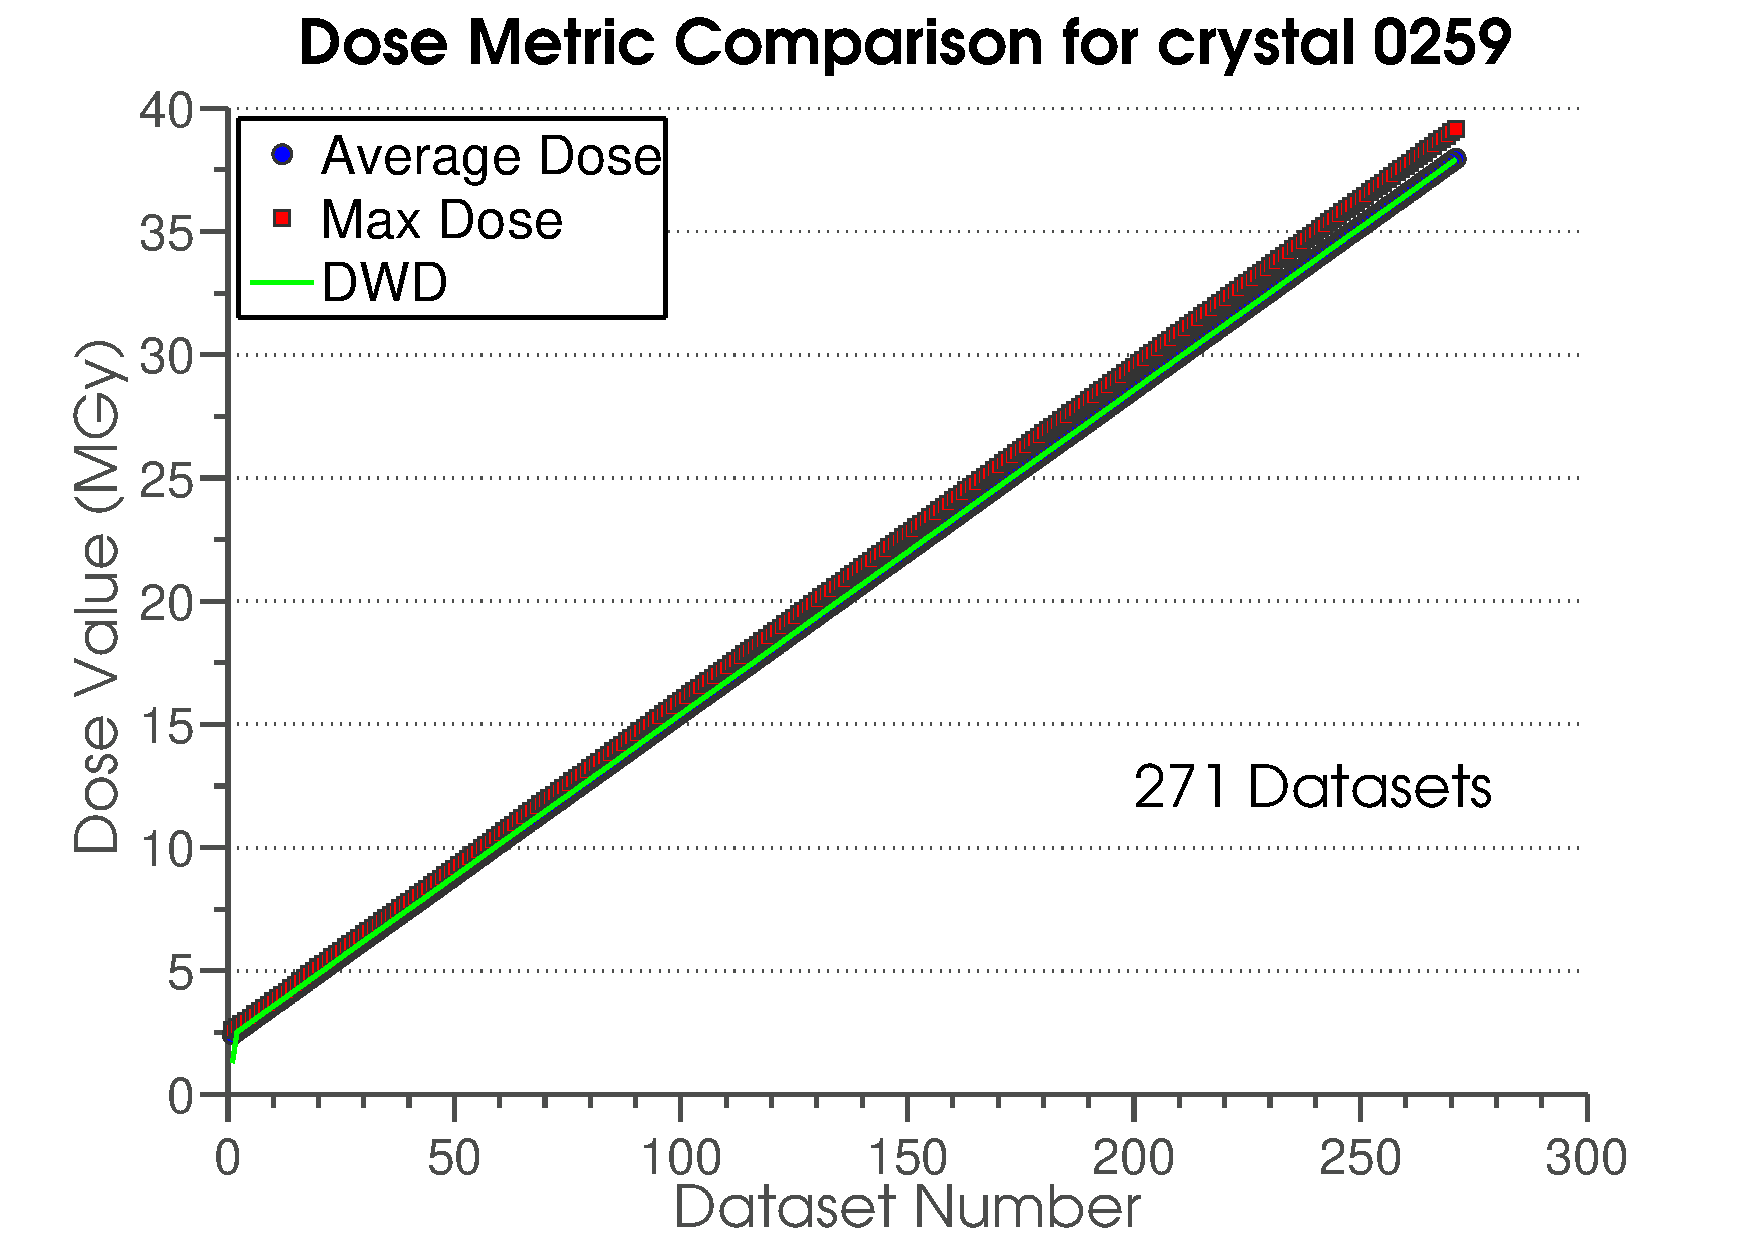
\includegraphics[width=\textwidth]{figures/dwd/metrics.pdf}
                \caption{}
                \label{fig:Metrics}
        \end{subfigure}
				\\
        \begin{subfigure}[b]{1\textwidth}
                \centering
                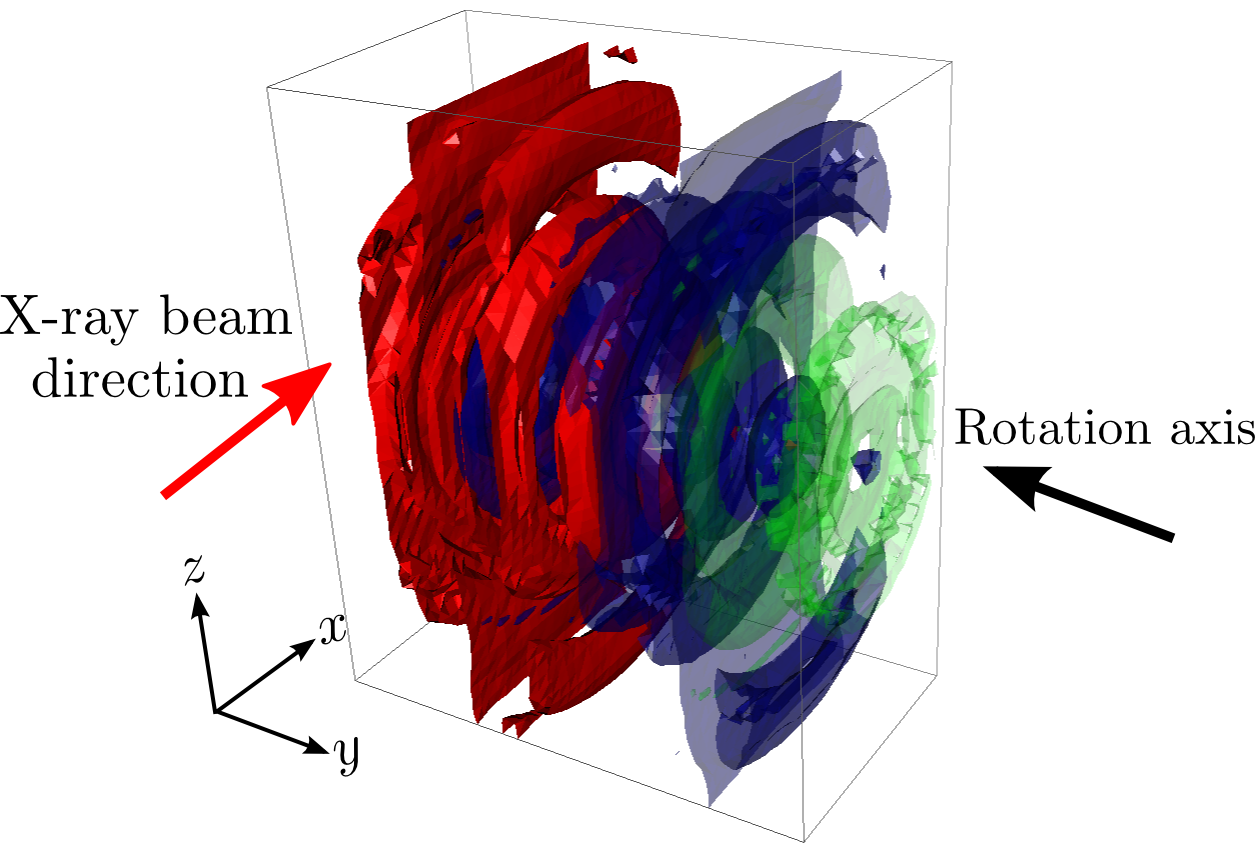
\includegraphics[width=\textwidth]{figures/dwd/raddose3d.png}
                \caption{}
                \label{fig:RADDOSE-3D dose contours uniform irradiation}
        \end{subfigure}
        \caption[Dose metrics and dose state of crystal showing uniform irradiation.]{(a) The three dose metric values are predicted to be very similar throughout the experiment.
        Here the DWD values are calculated using equation \ref{eq:DWD equation - no RDE}.
        (b) The calculated dose map from an MX simulation in RADDOSE-3D of an insulin crystal ($89\,\mu m \times 74\,\mu m \times 40\,\mu m$) exposed to the beam shown in Figure \ref{fig: Hamburg beam PGM} over a $1440^{\circ}$ rotation. The dose isosurfaces are: green $= 38\, MGy$, dark blue $= 38.5\, MGy$ and red $= 39\, MGy$. The dose distribution is very homogeneous.}
        \label{fig:Uniform}
\end{figure}

\subsection{Calculating the RDE}
\label{sub:Calculating the RDE}
To compare the theoretical RDEs calculated from the DDMs with the experimentally measured relative intensities, a spherically symmetric volume integral is performed on each of equations (\ref{eq: Sygusch and Allaire DDM}), (\ref{eq:Holton DDM}) and (\ref{eq:Leal DDM}) up to the resolution limit of the data (1.8$\,$\AA) at each of the recorded dose values.
These values are then divided by the same integral at dose $D =$ 0$\,$MGy to give an estimate of the relative intensities.
The resulting equations are given below and plotted in Figure \ref{fig:Relative Intensity Plots} along with the experimentally measured relative intensity values $I_n/I_1$ for the insulin crystals using the parameter values given in tables \ref{tab:RDE params1} and \ref{tab:RDE params2}.
\begin{align}
\text{RDE Holton} &= \f{\int^{h_{max}}_{h_{min}}{h^2 I_{ND}(h) \exp \left[ \f{- \ln(2) \times D \times h}{H}\right]}\, \dd h}{\int^{h_{max}}_{h_{min}}{h^2 I_{ND}(h)}\, \dd h} \label{eqrdeholt}\\[10pt]
\text{RDE Leal} &= \f{\exp\left[ -\gamma^2 D^2 \right] \int^{h_{max}}_{h_{min}}{h^2 J(h) \exp\left[ -\f{1}{2}(B_0 + \beta D)h^2\right]}\, \dd h }{\int^{h_{max}}_{h_{min}}{h^2 J(h) \exp\left[ -\f{1}{2} B_0 h^2\right]}\, \dd h }  \label{eqrdeleal}\\[10pt]
\text{RDE Sygusch} &= \f{\int^{h_{max}}_{h_{min}}{h^2 I(D=0,h) \left[ A_1(D) + A'_1(D) + A_2(D) \exp\left( \f{-B h^2}{2}\right)\right]}\, \dd h}{\int^{h_{max}}_{h_{min}}{h^2 I(D=0,h) \left[ A_1(0) + A'_1(0) + A_2(0) \exp\left( \f{-B h^2}{2}\right)\right]}\, \dd h} \label{eqrdesyg}
\end{align}
The root mean squared deviation (RMSD) was used to assess the fit of the RDE models to the data, with a lower RMSD suggesting a superior fit.
Although the parameter values were determined using only the data down to 70\% of the initial intensity, the RMSD values are found using the entire range of data for each crystal.
Figure \ref{fig:Relative Intensity Plots} shows that the RDE using the Leal \textit{et al.} intensity decay model best describes the crystal intensity decay for three out of the five crystals (crystal IDs: 0259, 137 and 128) according to the RMSD.
For the other two crystals (crystal IDs: 180 and 172), the RDE Sygusch model gives the lowest RMSD, suggesting that this model is also adequate at describing the relative intensity decay.
An important feature of the RDE Sygusch model is that it displays at least two phases during the relative intensity decay.
Both phases appear to decay linearly, with the first linear phase decaying faster than the second phase.
The RDE Holton model consistently gives the highest RMSD value for all five crystals and the decay curve does not correlate well visually with the decay shown in the data.

The RDE Leal model was chosen as the one to investigate with the DWD due to its simplicity and superior predictive ability.
Figure~\ref{fig:Relative Intensity - All crystals 1.4 Angstroms} shows the relative intensity values predicted by the RDE Leal model with parameters obtained as described in section \ref{sub:Obtaining Model Parameter Values} and averaged for each of the 5 insulin crystals processed.
However, this time the data were processed to a resolution limit of 1.4\,\AA\ (as opposed to the 1.8$\,$\AA\ limit used previously) to ensure that the difference in resolution would not affect the predictive ability of the model.
\begin{figure}[H]
    \centering
    \begin{subfigure}[b]{1\textwidth}
        \centering
        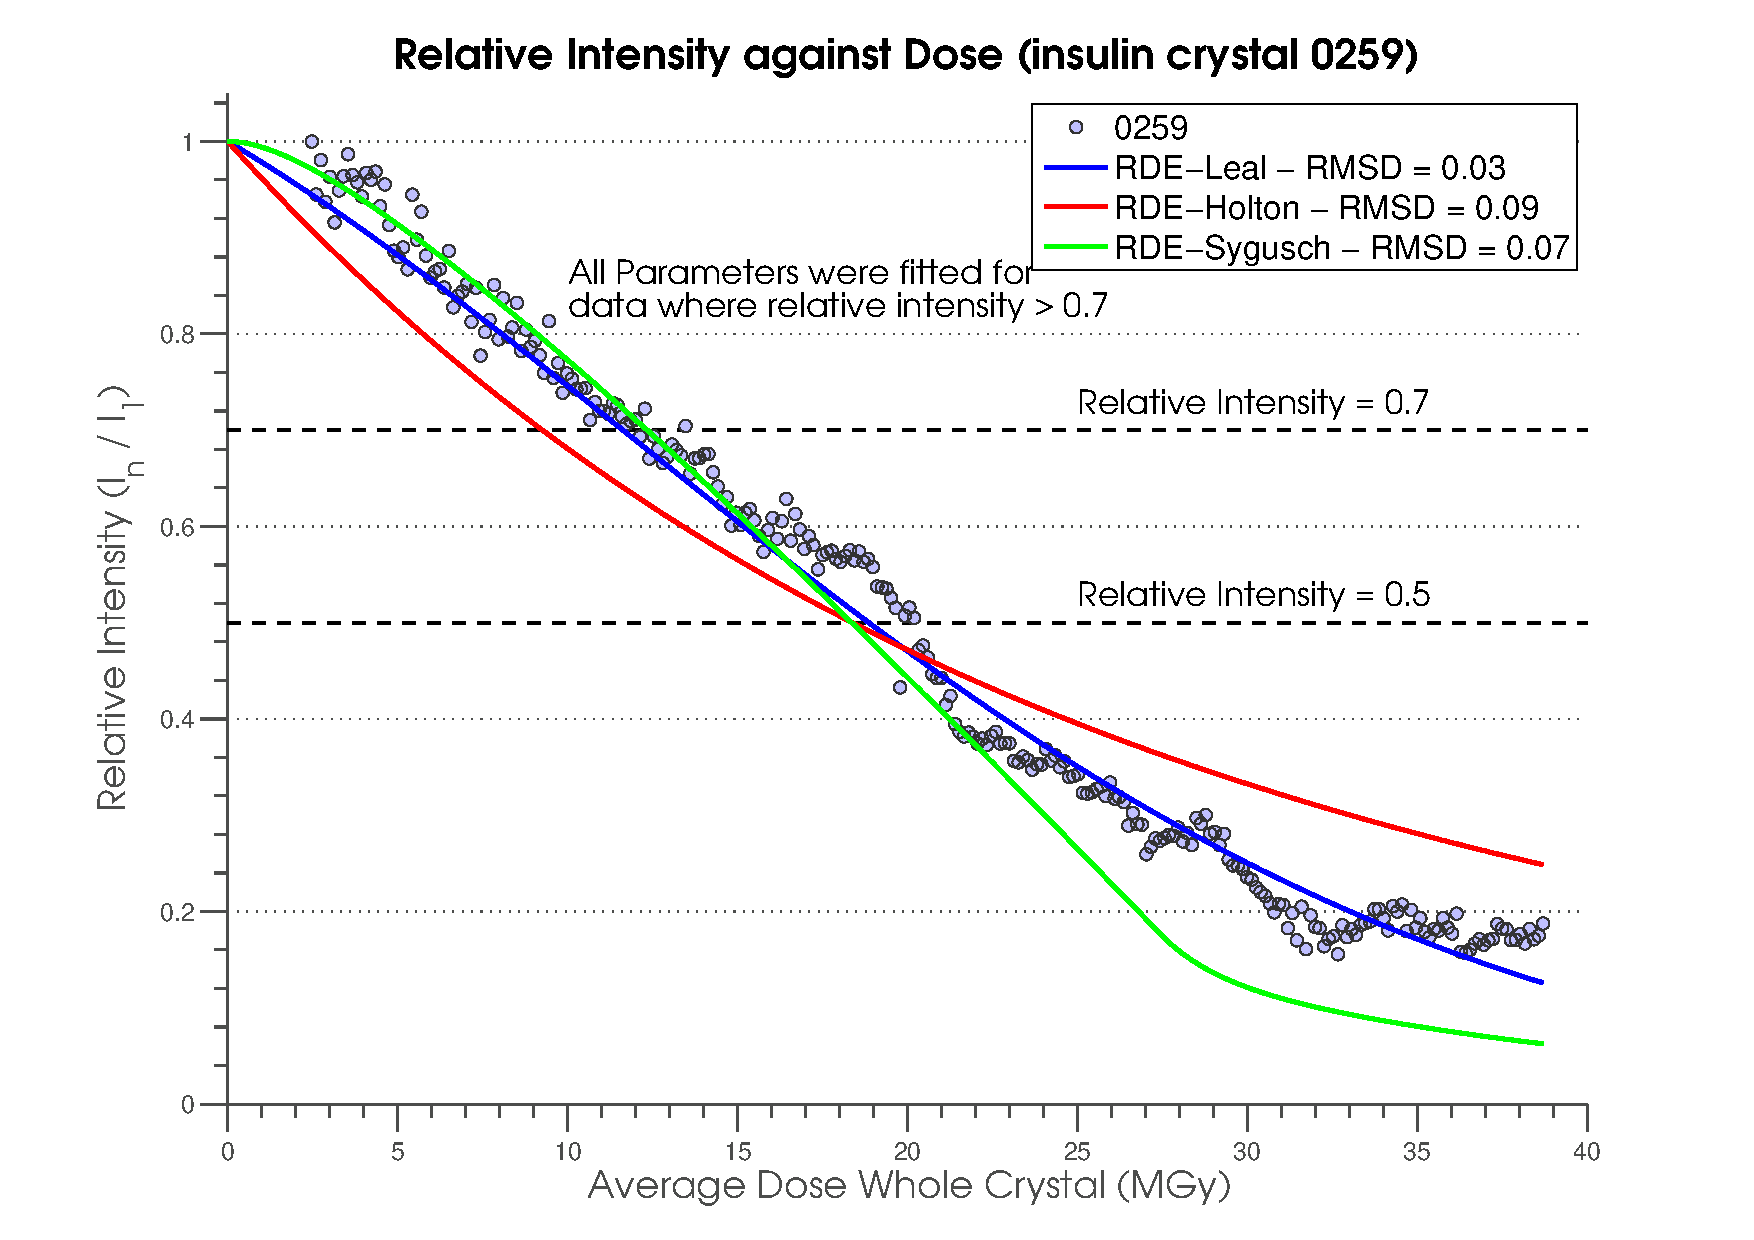
\includegraphics[width=\textwidth]{figures/dwd/relintplot0259.pdf}
        \caption{}
        \label{Relative Intensity Plots - 0259}
    \end{subfigure}
			\\
    \begin{subfigure}[b]{1\textwidth}
        \centering
        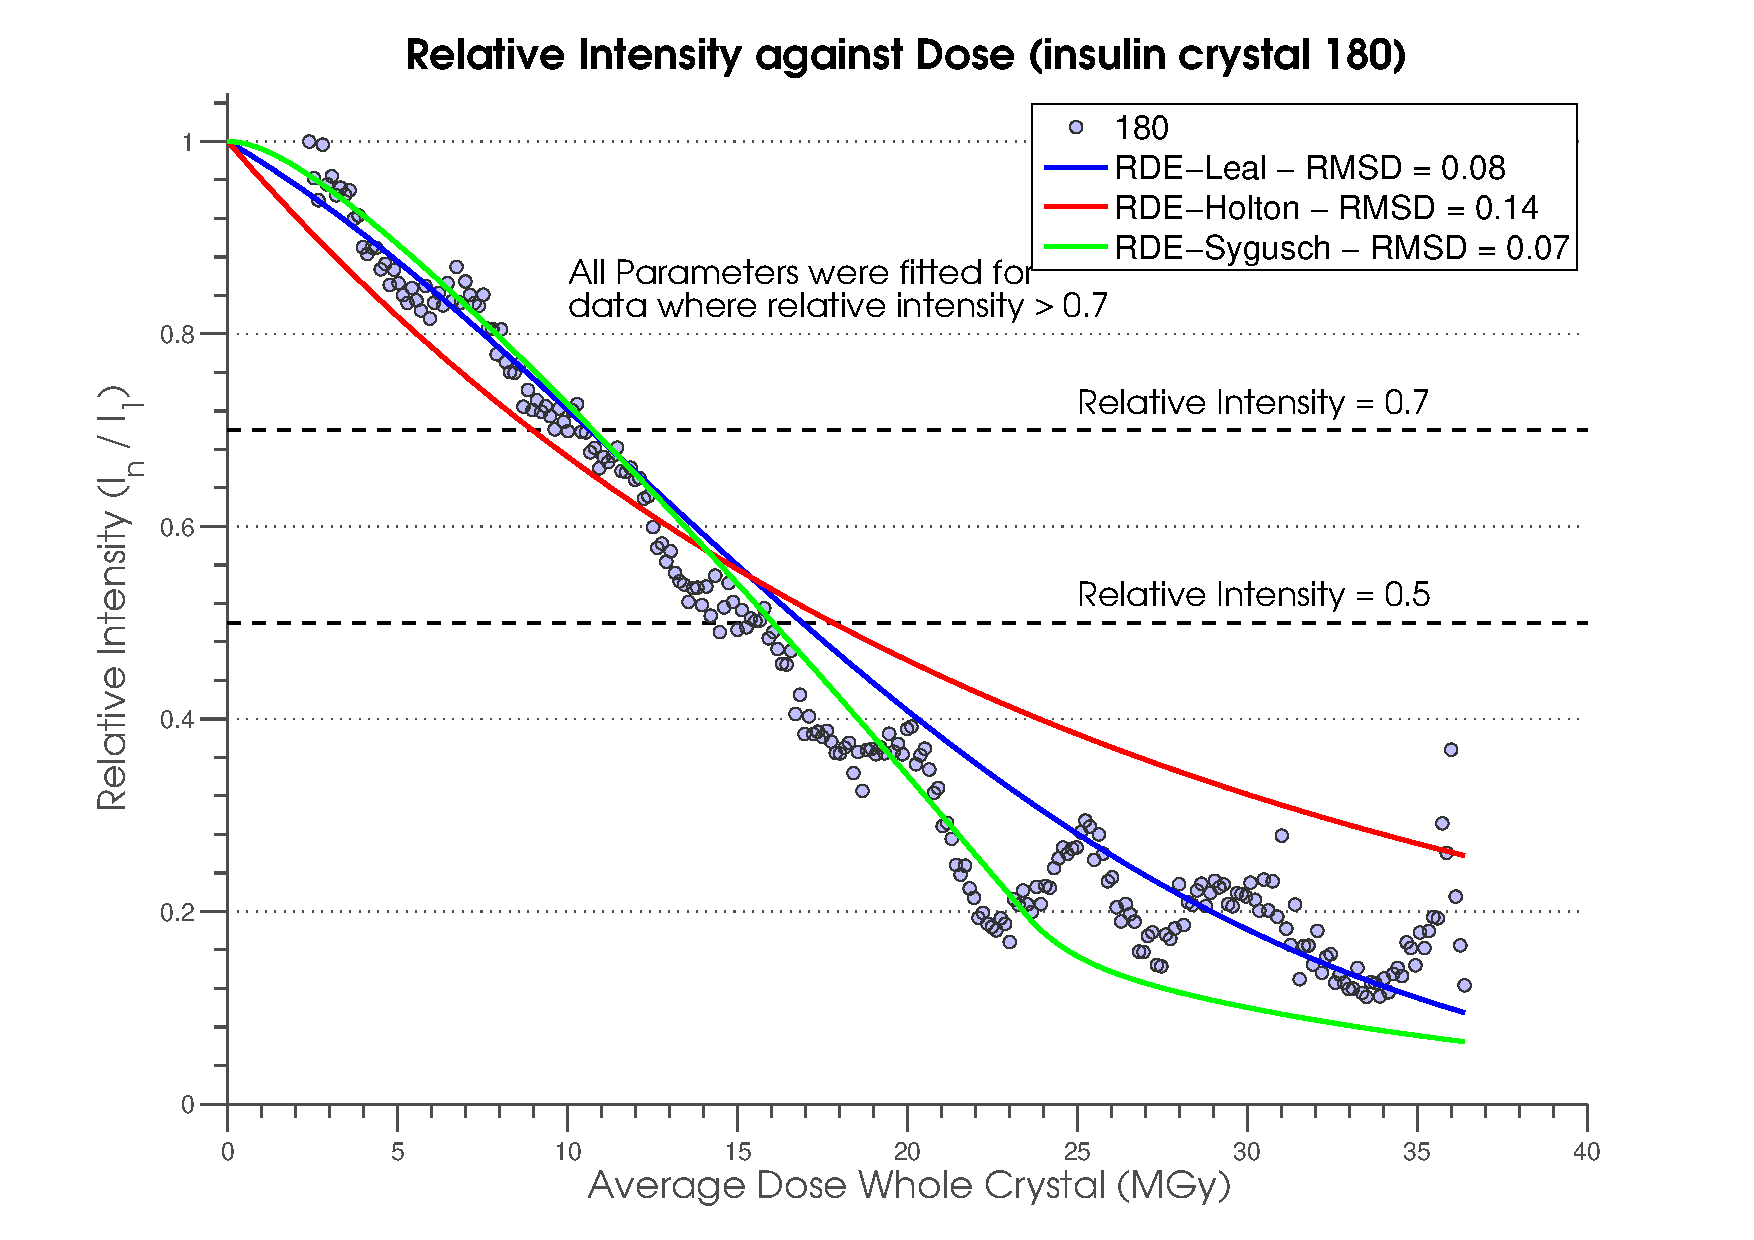
\includegraphics[width=\textwidth]{figures/dwd/relintplot180.pdf}
        \caption{}
        \label{Relative Intensity Plots - 180}
    \end{subfigure}
\end{figure}
\clearpage
\begin{figure}[H]
    \ContinuedFloat
    \centering
    \begin{subfigure}[b]{1\textwidth}
        \centering
        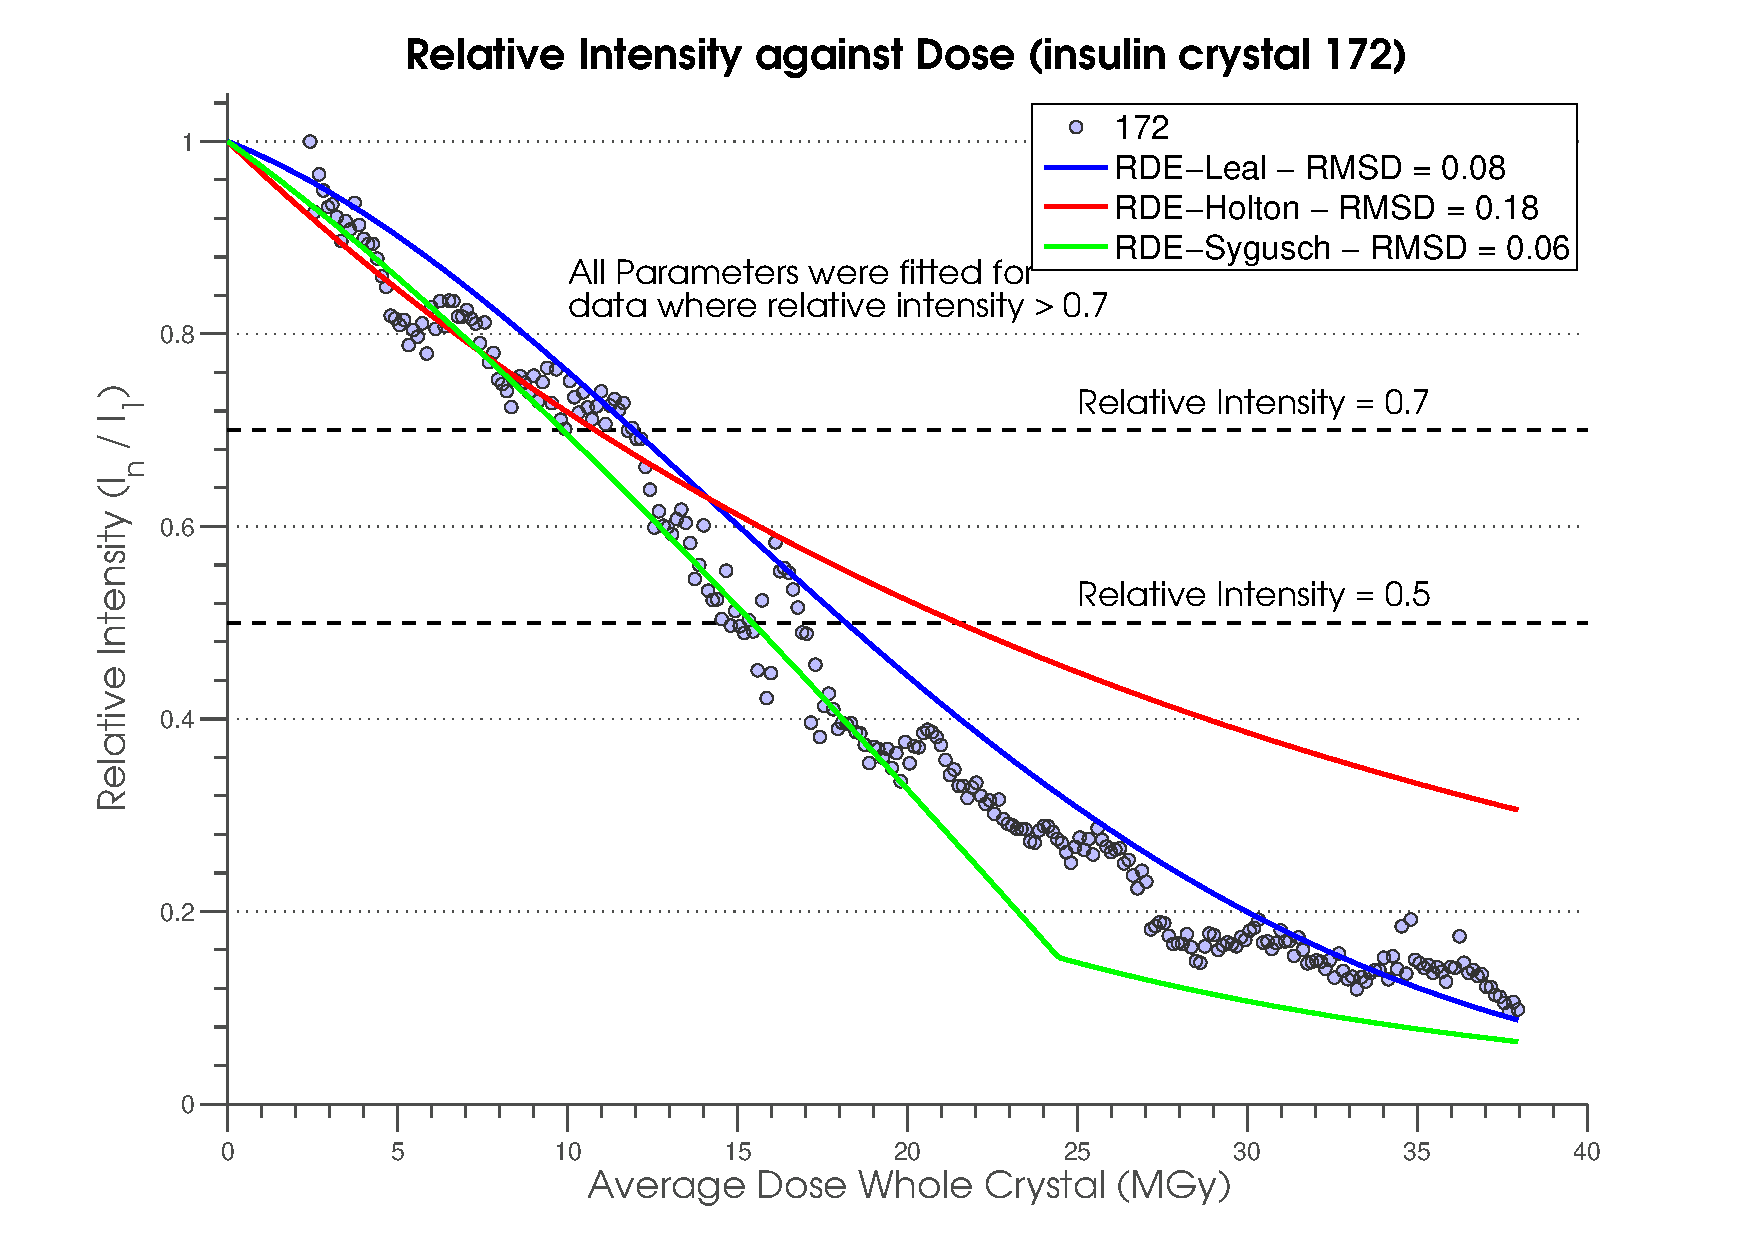
\includegraphics[width=\textwidth]{figures/dwd/relintplot172.pdf}
        \caption{}
        \label{Relative Intensity Plots - 172}
    \end{subfigure}
			\\
    \begin{subfigure}[b]{1\textwidth}
        \centering
        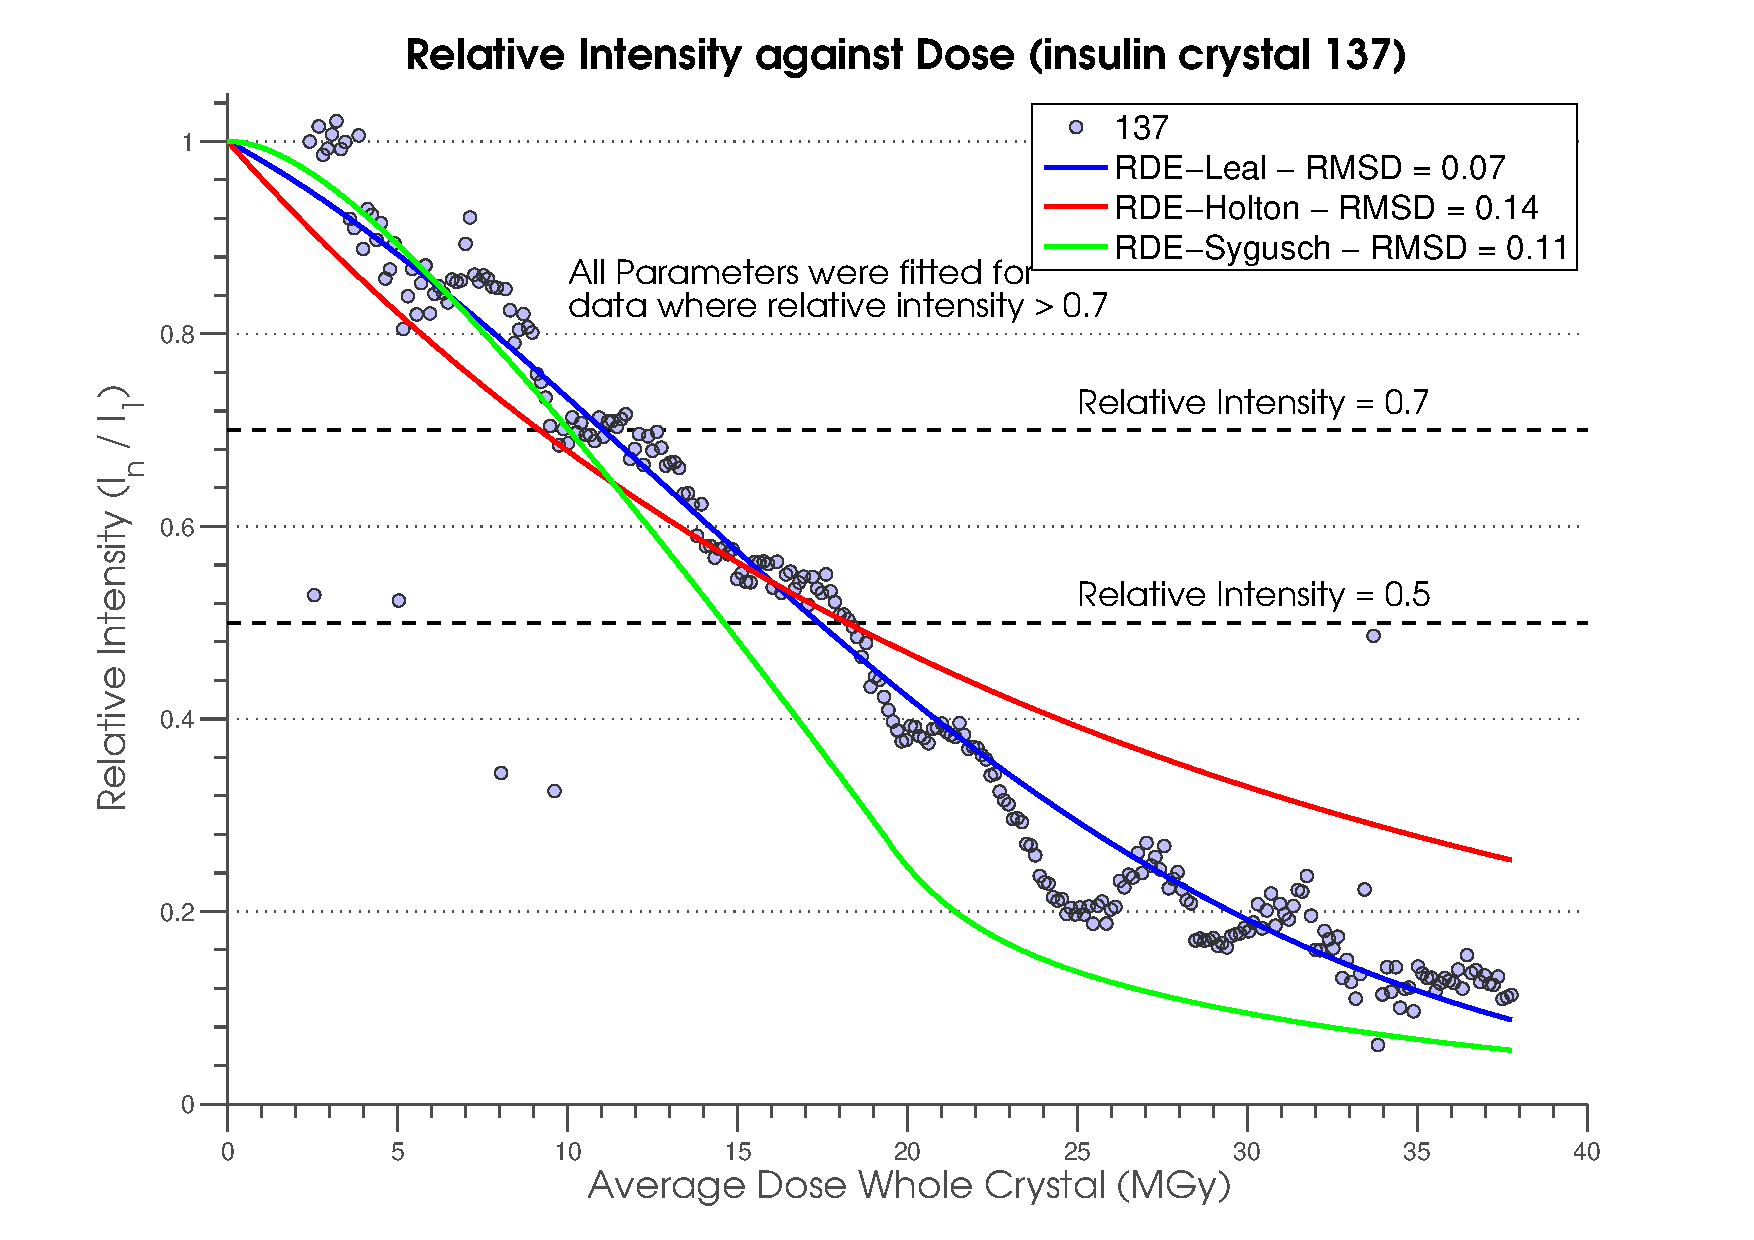
\includegraphics[width=\textwidth]{figures/dwd/relintplot137.pdf}
        \caption{}
        \label{Relative Intensity Plots - 137}
    \end{subfigure}
\end{figure}
\begin{figure}[H]
    \ContinuedFloat
    \centering
    \begin{subfigure}[b]{1\textwidth}
        \centering
        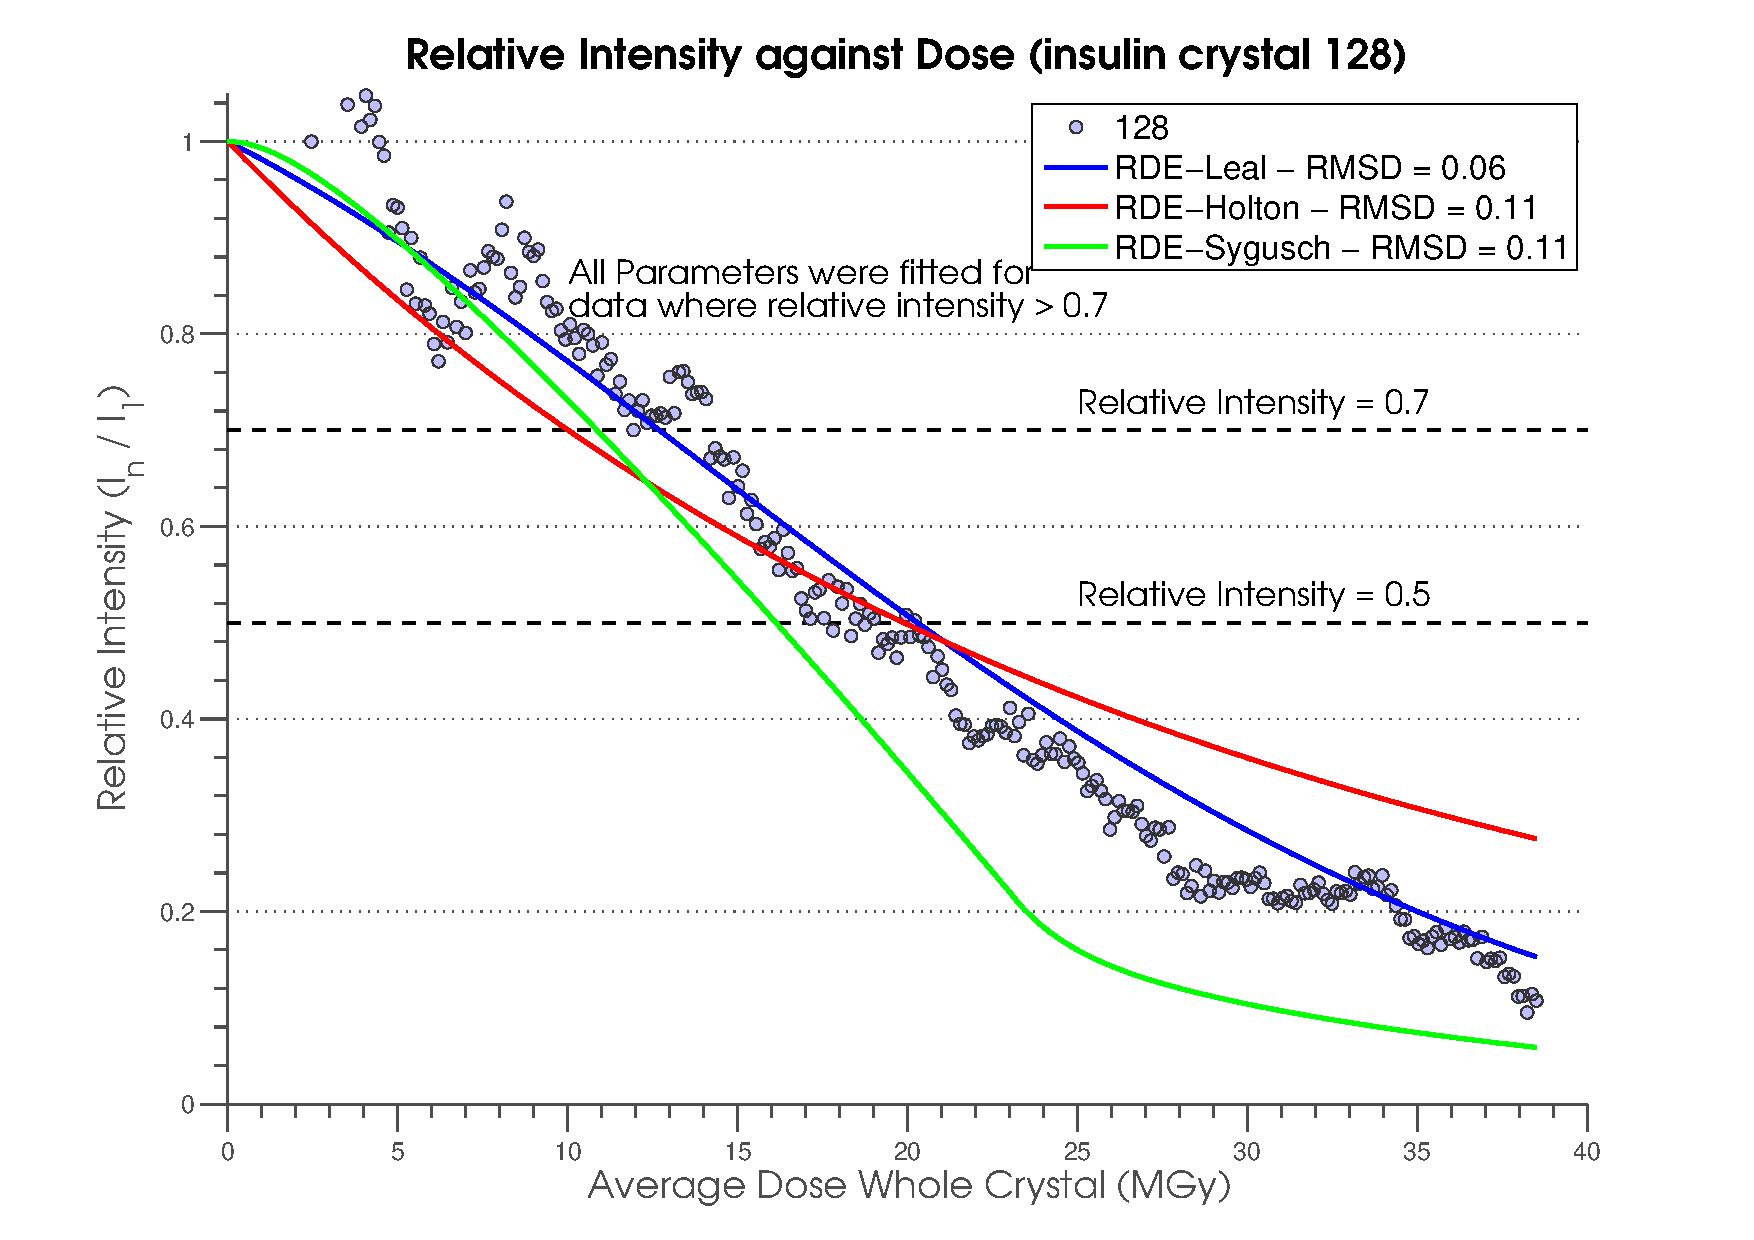
\includegraphics[width=\textwidth]{figures/dwd/relintplot128.pdf}
        \caption{}
        \label{Relative Intensity Plots - 128}
    \end{subfigure}
    \caption[Comparison of each dose decay model's ability to predict intensity decay for all insulin data.]{(a)-(e) Relative intensity plotted against the average dose over the whole crystal for each of the insulin crystals. Grey circles represent the experimental data processed to 1.8\,\AA. Blue, red and green solid lines represent the RDE-Leal, RDE-Holton and RDE-Sygusch models respectively. The RMSDs for each model are given in the figure legend on each plot.}
    \label{fig:Relative Intensity Plots}
\end{figure}

\begin{table}[H]
\small
\captionsetup{justification=centering}
	\caption[Best fit zero dose average intensity values for each resolution bin for the Holton dose decay model.]{Best fit zero dose average intensity values ($I_{ND} = I(D=0,h)$ (arb. units)) for each resolution bin. Note that $1/h_{mid} = d_{mid}$ where $d_{mid}$ is the mid-point resolution in each resolution bin}
	\centering
	\begin{tabular}{p{2cm} p{2cm} p{2cm} p{2cm} p{2cm} p{2cm}}
	\cline{2-6}
		& \multicolumn{5}{c}{Crystal ID} \\
		\hline
		resolution (\AA) ($1/h_{mid}$)	&	0259	& 180 		& 172 		& 137 		    & 128\\
		\hline
		12.53     				    &12984	    &8271 		&20087		    &29840		    &37536\\
		7.23     					&5161		&3342  		&7857			&12277		    &14732\\
		5.60     					&7764		&4946  		&11258		    &17550		    &21769\\
		4.74     					&11244	    &7043  		&15363		    &25479		    &31497\\
		4.18     					&12772	    &8000  		&18242		    &28230		    &35589\\
		3.78     					&11325	    &7050  		&16401		    &25625		    &31156\\
		3.47     					&8234		&5197  		&11827		    &19044		    &22606\\
		3.23     					&6035		&3787  		&9008			&13885		    &16543\\
		3.04     					&4293		&2673  		&6447			&9662			&11656\\
		2.87     					&3328		&2104  		&5075			&7592			&9092\\
		2.73     					&3021		&1904  		&4426			&6903			&8122\\
		2.61     					&2417		&1522  		&3569			&5509			&6473\\
		2.51     					&2232		&1369  		&3130			&4907			&5909\\
		2.41     					&1913		&1181  		&2697			&4261			&5101\\
		2.33     					&1659		&1010 		&2332			&3668			&4406\\
		2.25     					&1525		&959  		&2170			&3479			&3990\\
		2.18     					&1376		&853  		&1982			&3041			&3619\\
		2.12     					&1240		&746  		&1697			&2656			&3237\\
		2.06     					&958		&607  		&1341			&2159			&2451\\
		2.01     					&871		&540  		&1217			&1898			&2172\\
		1.96     					&719		&429  		&922			&1483			&1783\\
		1.91     					&645		&398  		&835			&1367			&1594\\
		1.87     					&524		&324  		&674			&1091			&1257\\
		1.83     					&422		&263  		&534			&891			&1041\\
		\hline
	\end{tabular}
	\label{tab:RDE params2}
\end{table}

\begin{table}[H]
\small
\captionsetup{justification=centering}
	\caption[Parameter values for the dose decay models.]{Parameter values for the dose decay models.
	Note: $K$ does not explicitly appear in equation (\ref{eqrdeleal}) and hence is not required for the analysis.
	The large $k_1$ parameter value for crystal 172 seems highly unphysical when compared with the other values.
	This large value implies that any site specific damaged crystal proportion in the crystal immediately becomes disordered, which suggests that the site specific state is present in negligible quantities for this crystal.
    Accounting for the intrinsic variability of crystals and the fact that the surface modification fraction of crystal 0259 was never higher than 5\% of the total crystal fraction, it is not too surprising that at least one of the crystals may show a negligible surface modification fraction.
	\newline
	units: $k'_0,\ k_1,\ k_2 \equiv MGy^{-1}, \quad H \equiv MGy\,\text{\AA}^{-1}, \quad B_0 \equiv \text{\AA}^2 \quad \beta \equiv \text{\AA}^2 MGy^{-1} \quad \gamma \equiv MGy^{-1}$}
	\centering
	\begin{tabular}{p{1.6cm} p{1.6cm} p{1.6cm} p{1.6cm} p{1.2cm} p{1.2cm} p{1.2cm} p{1.2cm}}
		\hline
		Crystal	&$k'_0$	& $k_1$	&$k_2$ &$H$	 &$B_0$	&$\beta$	&$\gamma$	\\
		\hline
		0259     &$3.6 \times 10^{-2}$   &$0.648$   	&$5.0 \times 10^{-2}$   &$5.466$    &$13.329$    &$0.383$  &$0.030$ \\
	  180      &$4.3 \times 10^{-2}$   &$0.772$   	&$5.0 \times 10^{-2}$   &$5.274$    &$13.408$    &$0.377$  &$0.036$ \\
		172      &$4.1 \times 10^{-2}$   &$2310$  &$5.0 \times 10^{-2}$   &$6.345$    &$14.818$    &$0.266$  &$0.037$ \\
	  137      &$5.1 \times 10^{-2}$   &$0.473$   	&$5.0 \times 10^{-2}$   &$5.391$    &$14.136$    &$0.353$  &$0.036$ \\
		128      &$4.3 \times 10^{-2}$   &$0.624$   	&$5.0 \times 10^{-2}$   &$5.842$    &$14.538$    &$0.338$  &$0.029$ \\
		\hline
	\end{tabular}
	\label{tab:RDE params1}
\end{table}

\begin{figure}
    \centering
    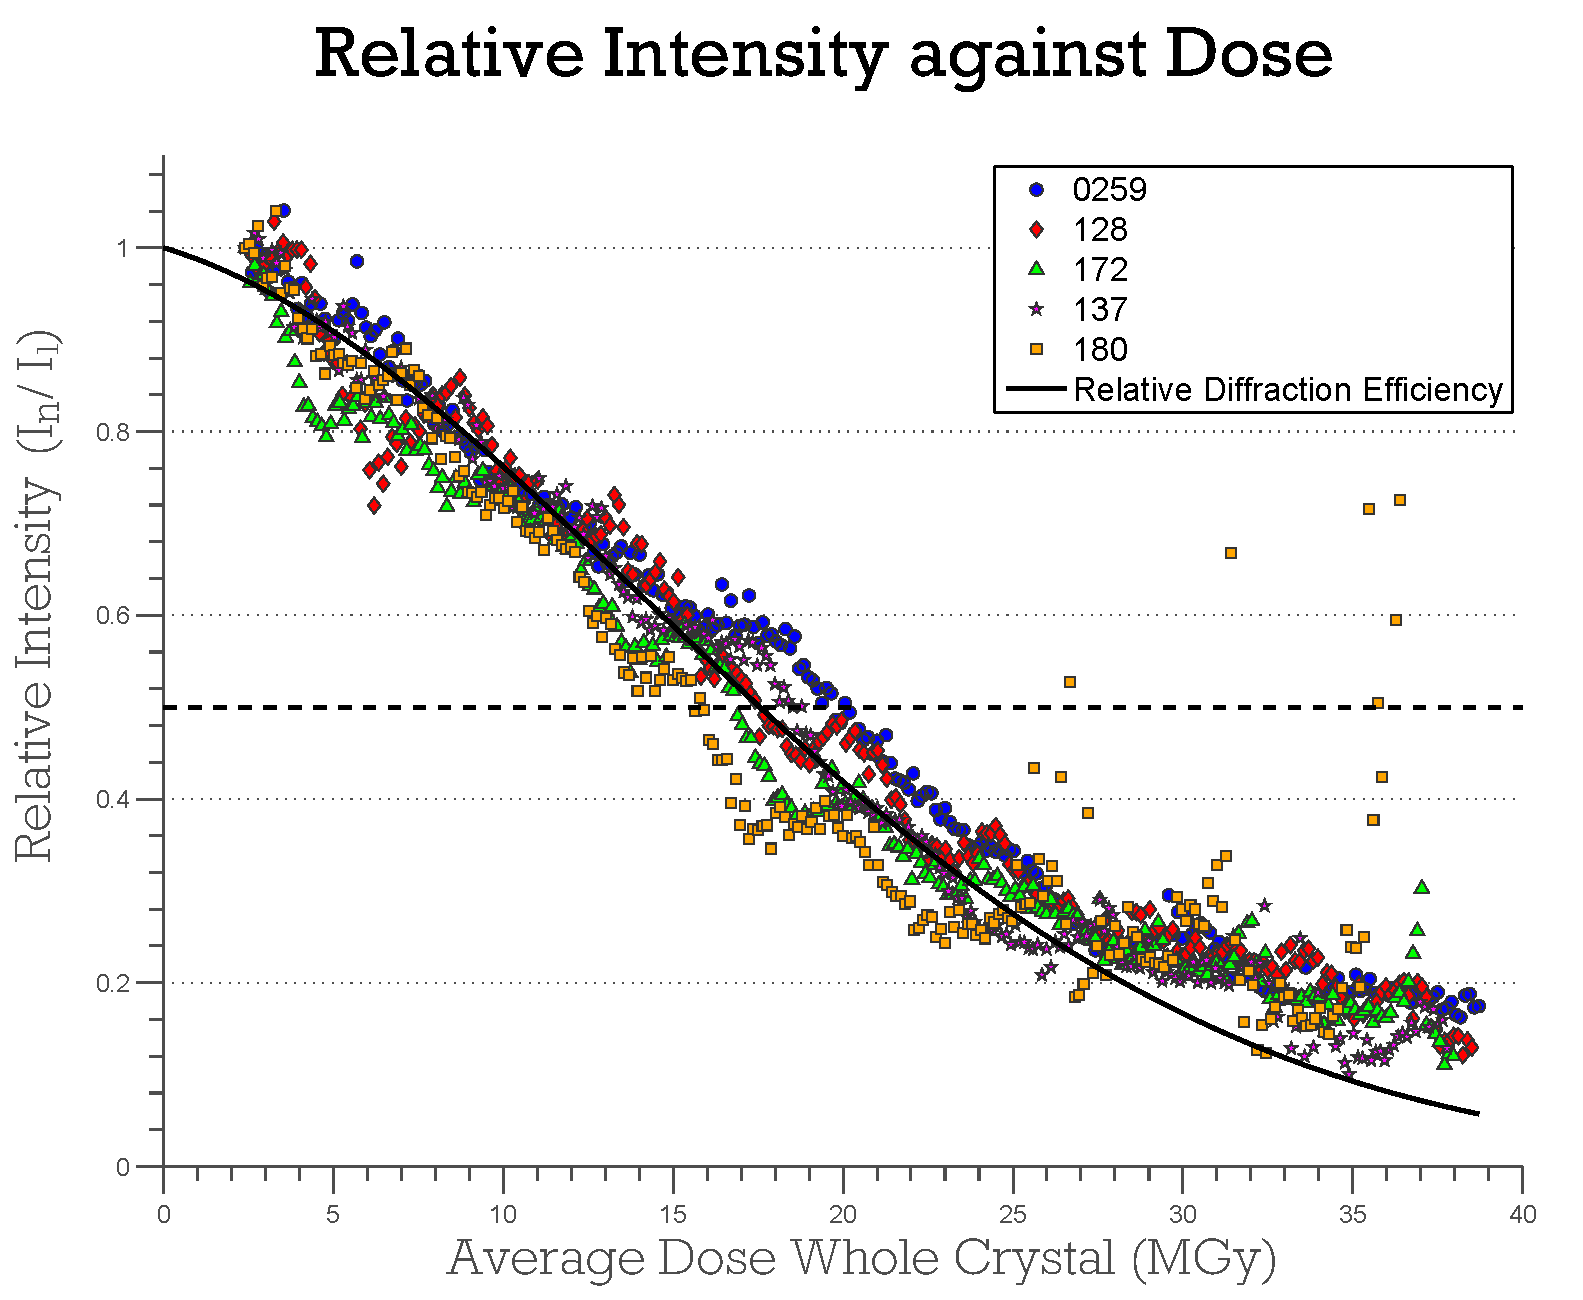
\includegraphics[width=1\textwidth]{figures/dwd/relintall_14A.pdf}
    \caption[Leal \textit{et al.} RDE model fitted to all insulin relative intensity data.]{Relative intensity plotted against the average dose over the whole crystal for all of the insulin crystals. Discrete data points represent the experimental data for each crystal processed to 1.4\,\AA. The black solid line is the RDE Leal model with parameters obtained as described in section \ref{sub:Obtaining Model Parameter Values} and with averaging of the parameter values for each crystal.}
    \label{fig:Relative Intensity - All crystals 1.4 Angstroms}
\end{figure}
